\chapter{Proposta do trabalho} \label{cap:proposta}

Conforme descrito na Introdução, este trabalho foi constituído de cinco etapas.
Neste capítulo é apresentado o resultado da segunda etapa que é a descrição da proposta do trabalho de acordo com os objetivos estabelecidos.
% 
% Para a plataforma ``Empurrando Juntos'', o lado servidor será implementado em uma aplicação chamada 
% Pentano\footnote{Repositório da aplicação: \url{https://gitlab.com/pentano/server}}.
% O Pentano será responsável por gerenciar as conversas, comentários, votos, agrupar os usuários
% e cuidar de todos os aspectos da autenticação das aplicações.
% 
\begin{figure}[h!]
\centering
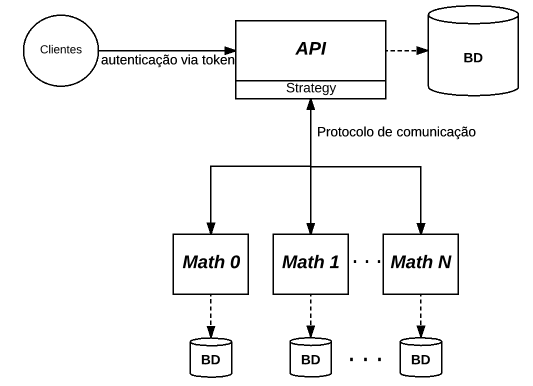
\includegraphics[scale=0.7]{figuras/esquema_pentano_2.png}
\caption{Estrutura do Pentano}
\label{fig:pentano}
\end{figure}
% 
% O Pentano pode ser abstraído em dois módulos principais, ilustrados na Figura \ref{fig:pentano}: o \textit{Server}, 
% que é o módulo responsável por prover os serviços para as aplicações; e o \textit{Math} que é o módulo responsável por realizar
% a clusterização, criando os grupos com os respectivos usuários.
% Portanto, a contribuição deste trabalho será a criação do módulo \textit{Server} do Pentano, que proverá serviços para realizar as
% propostas da plataforma ``Empurrando Juntos''.
% 
% \section{Requisitos da solução} \label{sec:requisitos}
% 
% Esta seção apresenta os requisitos funcionais e não funcionais identificados inicialmente para a aplicação.
% Os requisitos aqui apresentados foram considerados, inicialmente, para a solidificação e validação da arquitetura proposta.
% 
% \subsection*{Requisitos funcionais}
%   
%     Uma avaliação do escopo da plataforma ``Empurrando Juntos'' permitiu o levantamento de características desejadas do sistema e,
%     consequentemente, alguns requisitos associados, que foram sumarizados na Tabela \ref{tab:requisitos}.
% 
%     \begin{table}[h!]
%     \centering
%     \caption{Requisitos de alto nível da aplicação.}
%     \label{tab:requisitos}
%     \begin{tabular}{@{}cl@{}}
%     \toprule
%     \textbf{Característica}                      & \multicolumn{1}{c}{\textbf{Requisito}}                                                                                                \\ \midrule
%     \multirow{3}{*}{Gerenciamento de Usuário}    & O sistema deve permitir o cadastro de usuários                                                                                        \\
% 						& O sistema deve permitir a alteração de usuários                                                                                       \\
% 						& O sistema deve permitir a exclusão de usuários                                                                                         \\
%     \multirow{3}{*}{Gerenciamento de Conversa}   & O sistema deve permitir o cadastro de conversas                                                                                       \\
% 						& O sistema deve permitir a alteração de conversas                                                                                      \\
% 						& O sistema deve permitir a exclusão de conversas                                                                                       \\ \midrule
%     \multirow{4}{*}{Gerenciamento de Comentário} & O sistema deve permitir o cadastro de comentários em conversas                                                                        \\
% 						& O sistema deve permitir a alteração de comentários                                                                                    \\
% 						& O sistema deve permitir a exclusão de comentários                                                                                     \\ 
% 						& O sistema deve permitir que o usuário vote em comentários                                                                             \\ \midrule
%     Agrupamento de usuários                      & \begin{tabular}[c]{@{}l@{}}O sistema deve permitir a visualização dos usuários agrupados \\ de acordo com os votos dados\end{tabular} \\ \bottomrule
%     \end{tabular}
%     \end{table}
% 
% 
%  \subsection*{Requisitos não funcionais}
%     
%       O Pentano deve prover serviços para realizar os requisitos funcionais listados acima.
%       Estes serviços serão providos para a plataforma por meio de uma interface HTTP/HTTPS utilizando o estilo arquitetural REST.
%       
%       A autenticação e autorização das aplicações, e seus respectivos usuários, que utilizarão o Pentano deverá ser feita seguindo
%       o protocolo OAuth \footnotemark, visando uma maior escalabilidade da solução futuramente.
%       \footnotetext{OAuth Protocol. Disponível em \href{https://oauth.net/}{https://oauth.net}.}
%       
%       A tecnologia definida para implementação da solução proposta foi a linguagem Python juntamente com os \textit{frameworks}
%       Django e Django Rest Framework, utilizando o banco de dados PostgreSQL.
%       
%       Outro aspecto importante para esta aplicação é a questão da manutenibilidade, pois como será um software livre, a solução
%       deve ser desenvolvida de uma maneira que seja possível evoluir facilmente pela da comunidade.
%       Com isto em mente, foram definidos os seguintes padrões para o desenvolvimento da aplicação, considerando as tecnologias definidas:
%       utilização do PEP8 \footnotemark como folha de estilos e a utilização da especificação JSON API \footnotemark para formatação das respostas da API.
%       \footnotetext{Folha de estilos PEP8. Disponível em \href{https://www.python.org/dev/peps/pep-0008/}{https://www.python.org/dev/peps/pep-0008}.}
%       \footnotetext{Especificação JSON API. Disponível em \href{http://jsonapi.org/}{http://jsonapi.org}.}
%       
% \section{Arquitetura da solução}
% 
% Para contemplar os requisitos elicitados foram mapeadas as entidades principais e os relacionamentos entre elas. 
% As principais entidades que foram identificadas são Usuário, Conversa e Comentário. Um usuário pode criar
% conversas e comentários para cada conversa e participar de outras conversas, criadas por outros usuários.
% A participação de um usuário em uma conversa é dada pelo ato de criação de comentários naquela conversa ou
% no ato de votar em um comentário de uma conversa. Esse mapeamento é ilustrado na Figura \ref{fig:entidades}.
% 
% \begin{figure}[h!]
% \centering
% 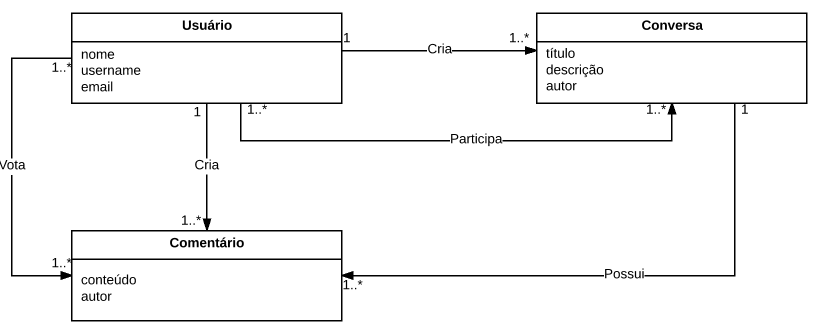
\includegraphics[scale=0.5]{figuras/entidades.png}
% \caption{Relacionamento das principais entidades da API}
% \label{fig:entidades}
% \end{figure}
% 
% Como o \textit{framework} Django foi escolhido como tecnologia de implementação da API, a arquitetura proposta foi pensada valendo-se de 
% recursos providos pelo própria arquitetura do \textit{framework}.
% No Django, uma aplicação web é abstraída como um projeto, e um projeto é composto por uma coleção de aplicações
% (ou, de forma abreviada, \textit{apps}) independentes, que
% são pacotes Python que proveem um conjunto de funcionalidades relacionadas e podem ser reutilizados \cite{django_apps}.
% Com o intuito de manter os \textit{apps} independentes e desacoplados o Django ainda conta com uma arquitetura de despache
% de sinais para que partes interessadas sejam notificadas de ações que ocorreram em outra parte da aplicação, permitindo uma comunicação
% desacoplada entre os \textit{apps} \cite{django_signals}.
% 
% Portanto, toda a solução foi componentizada utilizando \textit{apps} do 
% Django e parte da comunicação entre os \textit{apps} é feita através de sinais do Django, dentro do projeto \emph{Pentano}.
% Considerando os requisitos funcionais e não funcionais da solução, especificados anteriormente, a arquitetura da solução foi definida 
% conforme a Figura \ref{fig:arquitetura_api}, onde no módulo \textit{Server} temos dois \textit{apps} independentes, um responsável
% por cuidar de toda parte de autenticação da aplicação (\textit{app} de contas) e o outro para gerenciar as entidades apresentadas na
% Figura \ref{fig:entidades} (\textit{app} de conversas).
% 
% \begin{figure}[h!]
% \centering
% 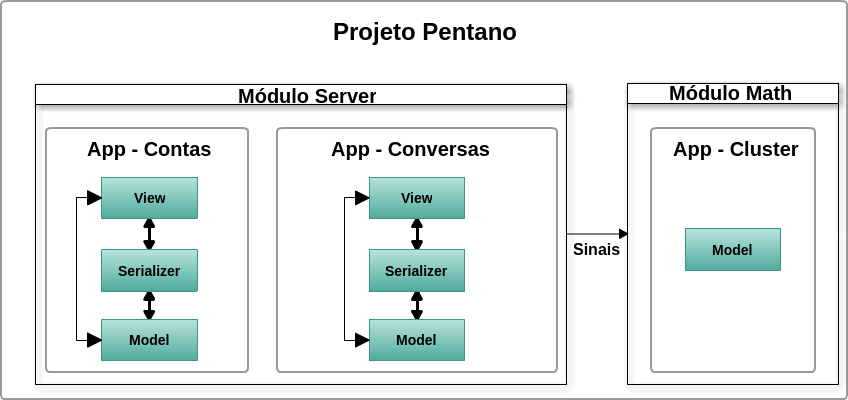
\includegraphics[scale=0.5]{figuras/arquitetura_api.png}
% \caption{Entidades da API}
% \label{fig:arquitetura_api}
% \end{figure}
% 
% 
% No módulo \textit{Server}, para cada \textit{app} foi definida uma arquitetura
% em 3 camadas: \textit{models}, \textit{views} e \textit{serializers}.
% A camada \textit{view} recebe e responde as requisições provenientes do cliente.
% A camada \textit{serializer} é responsável pelo tratamento e formatação dos dados das \textit{models}
% para renderização em JSON, seguindo a especificação JSON API.
% 
% Por fim, a camada \textit{model} contém aspectos negociais relacionados a cada uma das entidades definidas na 
% Figura \ref{fig:entidades}. Além disso, nessa camada é estabelecida a comunicação com o módulo de clusterização através de sinais.
% Os sinais criados são disparados durante as requisições de realização de novos votos e o módulo de clusterização é registrado
% como \textit{listener} desse evento, reagrupando os usuários quando um novo voto é cadastrado.
% 
% \vfill
% \pagebreak
% \begin{figure}[bt!]
% \centering
% 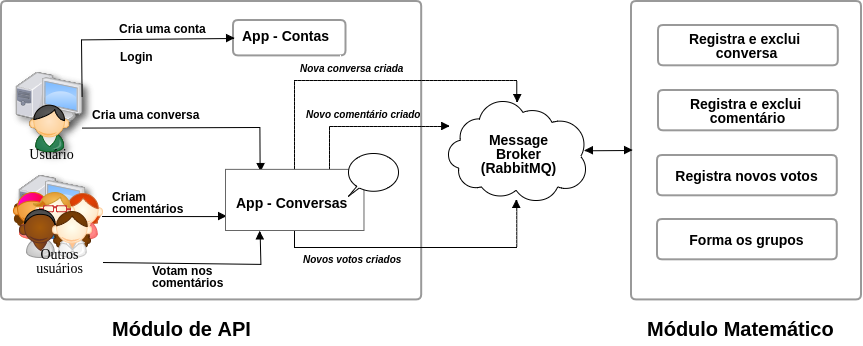
\includegraphics[scale=0.6]{figuras/resumo_ej_api.png}
% \caption{Funcionamento do Empurrando Juntos - Comunicação entre os módulos}
% \label{fig:resumo_ej_api}
% \end{figure}
% 
% 
% Na Figura \ref{fig:resumo_ej_api} é apresentado o fluxo de funcionamento do Empurrando Juntos de acordo com a arquitetura
% estabelecida para o Pentano. Inicialmente, um usuário faz o cadastro na aplicação, cuja requisição é tratada pelo \textit{app} de contas.
% Após a autenticação do usuário, ele pode criar conversas e comentários na aplicação. Outros usuários podem criar comentários e votar
% nos comentários. Todas essas operações relacionadas à conversas, comentários e votos são tratadas pelo \textit{app} de conversas.
% Quando um novo voto é realizado em algum comentário de uma conversa, o \textit{app} de conversas dispara um sinal informando que um novo
% voto foi criado. Esse sinal é recebido pelo \textit{app} de \textit{cluster}, que calcula novamente os \textit{clusters} considerando
% o usuário do novo voto, gerando novos grupos de usuários.

% \section{Resultados Esperados}


\begin{figure}[ht!]
\centering
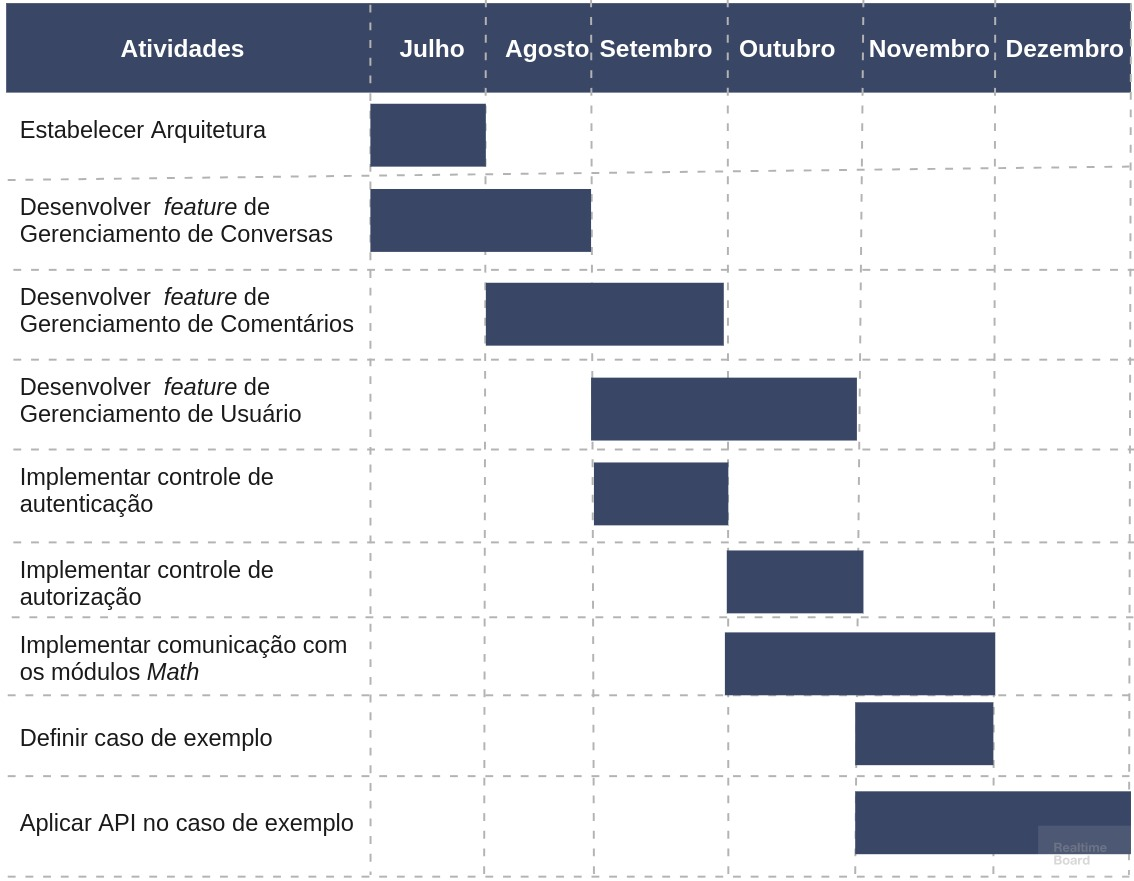
\includegraphics[scale=0.4]{figuras/cronograma.jpg}
\caption{Cronograma de execução do trabalho}
\label{fig:planejamento}
\end{figure}







